%+----------------------------------------------------------------------------+
%| SLIDES: 
%| Chapter: Observables - Hamiltonians - Symplectic structure
%| Author: Antonio miti
%| Event: Phd Colloquium - What is ... Geometric mechanics?
%+----------------------------------------------------------------------------+

%- HandOut Flag -----------------------------------------------------------------------------------------
\makeatletter
\@ifundefined{ifHandout}{%
  \expandafter\newif\csname ifHandout\endcsname
}{}
\makeatother

%- D0cum3nt ----------------------------------------------------------------------------------------------
\documentclass[beamer,10pt]{standalone}   
%\documentclass[beamer,10pt,handout]{standalone}  \Handouttrue  

\ifHandout
	\setbeameroption{show notes} %print notes   
\fi

	
%- Packages ----------------------------------------------------------------------------------------------
\usepackage{custom-style}
\usetikzlibrary{positioning}
\usepackage{multicol}
\usepackage[thinlines]{easytable}

%--Beamer Style-----------------------------------------------------------------------------------------------
\usetheme{toninus}
\usepackage{animate}
\usetikzlibrary{positioning, arrows}
\usetikzlibrary{shapes,shapes.callouts}

\begin{document}

%-------------------------------------------------------------------------------------------------------------------------------------------------
\begin{frame}{Observables}
	An observables is:
	\vfill
	\begin{columns}[T]
		\begin{column}{0.5\textwidth}
			\begin{itemize}
				\item a procedure to read a certain quantity (a number) out of any state of the system
				\item<2-> a quantity that can be measured with a device. 
			\end{itemize}				
			%
			\vspace{.5em}
			\onslide<3->{
				\begin{exblock}[Pendulum inclination]
					Measure the inclination of the rod with a goniometer.
				\end{exblock}			
			}
			%
			\vspace{.5em}
			\onslide<4->{
				\begin{mathblock}
					Observables are given by smooth functions on the phase space $M$:
					\begin{displaymath}
						\mathcal{O}=C^{\infty}(M)~.
					\end{displaymath}
				\end{mathblock}
			}
		\end{column}
		\begin{column}{0.5\textwidth}
			\begin{center}
				\ifHandout 
					\includegraphics<3>[width=.7\textwidth]{Pictures/observo}				
				\else
					\includegraphics<1>[width=.9\textwidth]{Pictures/pendo60-nogonio}
					\includegraphics<2>[width=.9\textwidth]{Pictures/pendo60}
					\includegraphics<3>[width=.9\textwidth]{Pictures/observo}
				\fi
				
				\only<3>{
					\tikz[overlay,remember picture]
					{
						\node[ellipse callout,fill=white!50,
			               draw=black,
			               anchor=base]            
			            	 (base) at ($(current page.east)+(-5,3)$) [rotate=-0,text width=1.5cm,align=center,callout relative pointer={(-.3,-.8)}] 
			            	 {Measure: \\$\theta=\pi/3$\\$\phantom{\theta}\cong 1.05$};
					}	
				}
				\only<4>{
					\resizebox{.9\textwidth}{!}{				
						\begin{tikzpicture}
							\pgfmathtruncatemacro\steps{4}
							\pgfmathtruncatemacro\mintheta{-120}
							\pgfmathtruncatemacro\maxtheta{-60}
							\pgfmathsetmacro\deltatheta{(\maxtheta-\mintheta)/(\steps)}
							\pgfmathsetmacro\viewpitch{30}
							\pgfmathsetmacro\diam{2}
							\pgfmathsetmacro\H{4}
							\pgfmathsetmacro\deltaH{(\H)/(\steps)}
							\pgfmathsetmacro\X{\diam}
							\pgfmathsetmacro\Y{\diam*sin(\viewpitch)}	
							\pgfmathsetmacro\vel{\diam/4}	
		
							\draw[green,dashed,fill=green!20] (0,0) ellipse ({\X} and {\Y});
							%\draw [blue,dashed] (-1.25,-3.5) arc (180:360:1.25 and -0.5);
							\draw[green,dashed,fill=green!20] (0,-{\H}) ellipse ({\X} and {\Y});
							\draw [blue,dashed] (-{\X},-{.5*\H}) arc (180:360:{\X} and -{\Y});
							\draw [green](-{\X},0) -- (-{\X},-{\H});
							\draw [green]({\X},-{\H}) -- ({\X},0);  
							\fill [green!80,opacity=0.5] (-{\X},0) -- (-{\X},-{\H}) arc (180:360:{\X} and {\Y}) -- ({\X},0) arc (0:180:{\X} and -{\Y});
							\draw [blue](-\X,-{.5*\H}) arc (180:360:{\X} and {\Y});

							\foreach \i in {0,1,...,\steps}{
								\pgfmathsetmacro\h{-\i*\deltaH}
								\pgfmathsetmacro\theta{\mintheta + \i*\deltatheta}	
								\pgfmathsetmacro\thetalabel{-\theta -90}	
									
								\draw[red,-stealth] (0,\h)++({cos(\theta)*\X},{sin(\theta)*\Y}) node[draw,cross out]{}  -- (5,{pi*2*(\thetalabel)/180-\H/2})node[right] {${\thetalabel}^\circ$};
							}
							\draw[->] (5,-{\H})--(5,0) node[above] {${\Theta}$}; % ordinate
						\end{tikzpicture}	
					}
				}
			\end{center}
		\end{column}
	\end{columns}
\end{frame}
\note[itemize]{
	\item Observation /Measure, procedure to extract a number from a physical system.	E.g. a measure with a device	

}
%-------------------------------------------------------------------------------------------------------------------------------------------------

%-------------------------------------------------------------------------------------------------------------------------------------------------
\begin{frame}[t]{Hamiltonian: Energy observable}
	A certain observable takes a central role:
	\vfill
	\begin{columns}[T]
		\begin{column}{0.5\textwidth}
			\begin{defblock}[Hamiltonian observable]
				Observable measuring the total energy of the system.
				\begin{displaymath}
					H = \text{Kinetic} + \text{Potential}
				\end{displaymath}
			\end{defblock}		
			\vspace{1em}
			\onslide<2->{
				\begin{exblock}[Pendulum]
					In practical terms: $H$ is a device measuring the battery charge dissipated by a motor to lift the bob to a certain height.	
				\end{exblock}
			}			
			%
		\end{column}
		\begin{column}{0.5\textwidth}
			\begin{center}
				\onslide<2->{	
					\animategraphics[autoplay,palindrome,width=\textwidth]{1}{Pictures/pendolabenergy-}{0}{1}
				}			
			\end{center}
		\end{column}
	\end{columns}
	\vfill
	\onslide<3->{
		\begin{upshotblocksimp}
			Upshot: $H$	embodies how the ambient acts on the system and the system's inertia to respond to the external forces.
		\end{upshotblocksimp}		
	}


\end{frame}
\note[itemize]{
	\item among all possible observables "Energy" has a pivotal role:
	\item Without being too philosophica. Consider our pendulum system.
	\item \emph{potential energy} account the interaction of the "ambient" with the "body".
	\item \emph{kinetic energy} is the energy of the motion.
}
%-------------------------------------------------------------------------------------------------------------------------------------------------

%-------------------------------------------------------------------------------------------------------------------------------------------------
\begin{frame}{Symplectic structure - an intuition -}
	\center
	\alert{Phase spaces has a canonical \underline{symplectic structure}}
	\vfill
	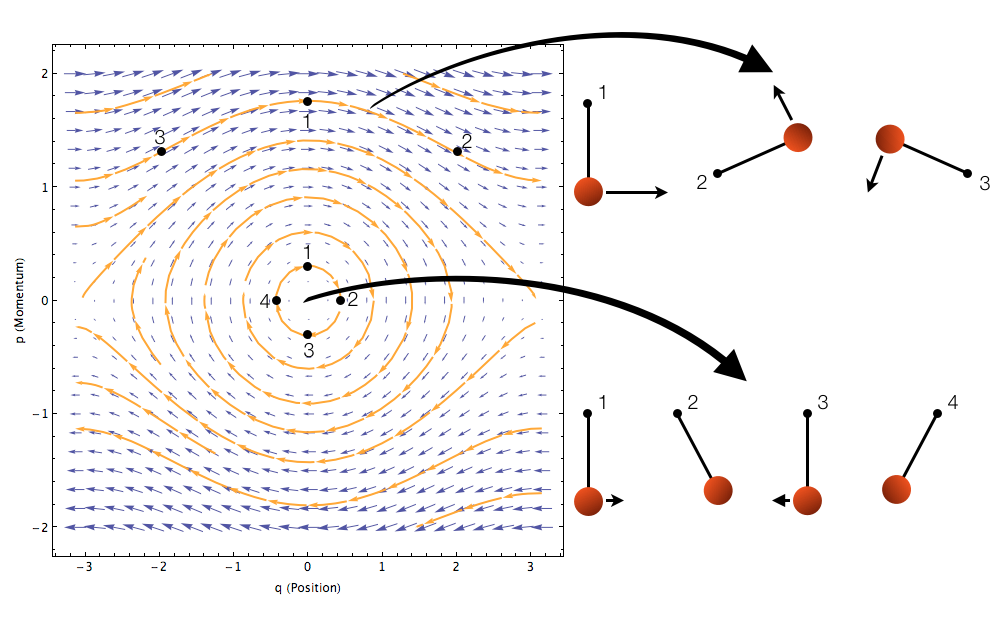
\includegraphics[width=.85\textwidth]{Pictures/pendo-hamiltonianfield}	
	\vfill
	\begin{itemize}
		\item Is  a prescription of an \emph{Hamiltonian field} $v_f$ to any observable $f$.
		\item The flow gives the evolution of the system when taking $f$ as the Hamiltonian.
		\item The Hamiltonian generates the \emph{time evolution}.
	\end{itemize}


\end{frame}
\note[itemize]{
	\item canonical i.e independent from arbitrary choices.
	\item the symplectic structure prescribes a tangent vector field to any observable quantity.
	\item integrate the flow implies to solve an ODE (a PDE if $M$ is $\infty$-dimensional).
		\begin{equation}
			\dot{q} = \dfrac{\partial H}{\partial p}
			~,\qquad 
			\dot{p} = - \dfrac{\partial H}{\partial q}
			\tag{Hamilton equations}	
		\end{equation}
	 \item Computing these solutions is where the analytical side of mechanics kicks in.
}
%-------------------------------------------------------------------------------------------------------------------------------------------------

%-------------------------------------------------------------------------------------------------------------------------------------------------
\begin{frame}{Quick reminder: Vector fields and differential forms}
\begin{TAB}(r,1cm,2cm)[5pt]{|c|c|c|}{|c|c|c|c|}% (rows,min,max)[tabcolsep]{columns}{rows}
 & Vector fields & Differential forms   \\
Informally & 
\parbox[t][][t]{4.25cm}{Smooth association of a vector $v\in T_p M$ for any $p\in M$} & 
\parbox[t][][t]{4.25cm}{Smooth association of a $k$-linear form on $T_p M$ for any $p \in M$} \\
Notation & 
\parbox[t][][t]{4.25cm}{$\mathfrak{X}(M)$} &
\parbox[t][][t]{4.25cm}{$\Omega^k(M)$} \\
Formal Definition& 
\parbox[t][][t]{4.25cm}{$\mathfrak{X}(M) = Der(C^\infty(M))$\\(Module of derivations on the algebra $C^\infty(M)$) } &
\parbox[t][][t]{4.25cm}{$Hom(\mathfrak{X}^{\otimes k}(M),C^\infty(M))$} \\
\end{TAB}


\end{frame}
\note[itemize]{
	\item 	Def symplectic structure 
	\item 	Canonical symplectic structure.	
}
%-------------------------------------------------------------------------------------------------------------------------------------------------


%-------------------------------------------------------------------------------------------------------------------------------------------------
\begin{frame}{Symplectic geometry in a nutshell}
\begin{columns}[T]
	\begin{column}{.50\linewidth}
		\centering
		\textit{ "geometric approach" to mechanics \dots}
		%
		\begin{columns}
			\begin{column}{.50\linewidth}
				\begin{center}
					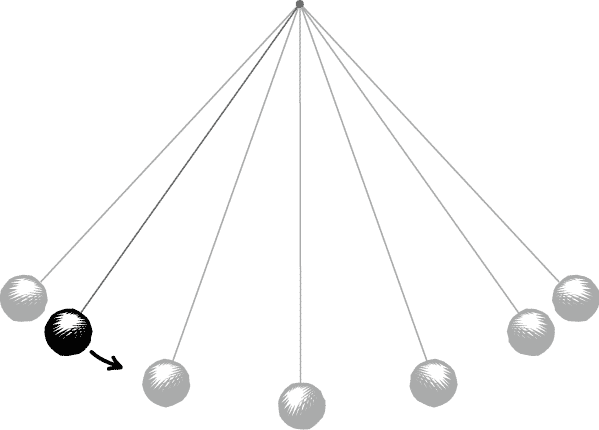
\includegraphics[width=0.8\linewidth]{Pictures/pendulum13}			
				\end{center}
			\end{column}	
			\begin{column}{.50\linewidth}
				\begin{center}
					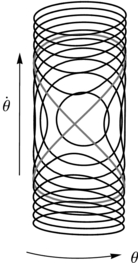
\includegraphics[width=0.45\linewidth]{Pictures/pendulum-phase-space}			
				\end{center}
			\end{column}	
		\end{columns}
		%
		\begin{defblock}[Symplectic Manifold]
			\includestandalone[width=0.95\textwidth]{Pictures/Figure_sym}	
		\end{defblock}
		%
		\begin{exblock}[$M = T^\ast Q$ is symplectic]
			$\omega = d \theta $ with
			$$ \left.\theta\right\vert_{(q,p)} (v) = p (\pi_\ast v) ~.$$
		\end{exblock}
	\end{column}
	\vrule{}
	\pause
	\begin{column}{.50\linewidth}
		\centering
		\textit{ "algebraic approach" to mechanics \dots}
		\vspace{1em}	
		\begin{defblock}[Classical Observables]
			Unital, associative, commutative algebra $C^\infty(M)$.
		\end{defblock}
		%
		\vspace{1em}
		\pause
		\begin{defblock}[Hamiltonian vector fields]
			$v_f \in \mathfrak{X}(M)$ such that:
			$$\iota_{v_f} \omega = -df \quad \text{(exact)}$$ %$\in B^1(M)$
			\small$v_f$ = \emph{Ham.v.f. pertaining to $f\in C^\infty(M)$}.
		\end{defblock}
		%
		\begin{defblock}[Poisson Algebra of Observables]
			$C^\infty(M)$ is a Poisson algebra with
			$$\{f,g\} = \iota_{v_g} \iota_{v_f} \omega = \omega(v_f,v_g) ~.$$
		\end{defblock}
	\end{column}
\end{columns}
\end{frame}
\note[itemize]{
	\footnotesize

	\item We work in the framework of multisymplectic geometry which is one of the possible generalizations of the well-established field of symplectic geometry.
	
	\item To recall what symplectic geometry is let me assume a particular point of view: mechanics.
	\\
	Idea:"
	Symplectic geometry is a branch of differential geometry studying symplectic manifolds; it originated as a formalization of the mathematical apparatus of classical mechanics and geometric optics."{\href{https://ncatlab.org/nlab/show/symplectic+geometry}{nlab}}
	
	Namely, a sym. mfd. is the geometric structure encoding the phase space of conservative, ordinary, classical, mechanical systems.
	
	\item $\theta$ = \emph{tautological 1-form}.
		$\theta$ evaluated at $p\in T^*Q$ in the fibre of $q\in Q$ and contracted with $v$ coincides with the form $p$ evaluated at $q$ and contracted with the push forward of $v$.
	
	\item We identify a special class of vector fields.
		Out of them one can define a Lie bracket.
	
	\item Poisson is a Lie algebra with the extra property of compatibility with the associative product (Leibniz rule)
}
%-------------------------------------------------------------------------------------------------------------------------------------------------

%------------------------------------------------------------------------------------------------
\begin{frame}{Syplectic geometry of the pendulum}\label{frame:symgeompendu}
  \begin{columns}[T]
   	\begin{column}{.35\textwidth}
   		\center
   		\vspace{-1em}
		\resizebox{.9\textwidth}{!}{
			\pgfmathtruncatemacro\steps{7}
			\pgfmathtruncatemacro\mintheta{-170}
			\pgfmathtruncatemacro\maxtheta{-30}
			\pgfmathsetmacro\deltatheta{(\maxtheta-\mintheta)/(\steps-1)}
			\pgfmathsetmacro\viewpitch{15}
			\pgfmathsetmacro\diam{2}
			\pgfmathsetmacro\H{2}
			\pgfmathsetmacro\deltaH{.5}
			\pgfmathsetmacro\X{\diam}
			\pgfmathsetmacro\Y{\diam*sin(\viewpitch)}	
			\pgfmathsetmacro\vel{\diam/4}	
					\begin{tikzpicture}
						\draw[green,dashed,fill=green!20] (0,0) ellipse ({\X} and {\Y});
						%\draw [blue,dashed] (-1.25,-3.5) arc (180:360:1.25 and -0.5);
						\draw[green,dashed,fill=green!20] (0,-{\H}) ellipse ({\X} and {\Y});
						\draw [blue,dashed] (-{\X},-{.5*\H}) arc (180:360:{\X} and -{\Y});
						\draw [green](-{\X},0) -- (-{\X},-{\H});
						\draw [green]({\X},-{\H}) -- ({\X},0);  
						\fill [green!80,opacity=0.5] (-{\X},0) -- (-{\X},-{\H}) arc (180:360:{\X} and {\Y}) -- ({\X},0) arc (0:180:{\X} and -{\Y});
						\draw [blue](-\X,-{.5*\H}) arc (180:360:{\X} and {\Y});

			\draw [black,-Latex](-\X,-{1.25*\H}) arc (180:355:{\X} and {\Y}) node[midway,below]{$\theta$};
			\draw [black,-Latex](-{1.25*\X},-{\H}) -- 
			node[left] {$p$}	 (-{1.25*\X},0);
					\end{tikzpicture}	
		}   	   	
   	
   	
   	
    \end{column}
    \begin{column}{.65\textwidth}	
		\begin{itemize}
			\item $M=T^\ast S^1\cong S^1\times \mathbb{R} \sim (\theta, p_\theta)$
			\item two coordinates charts
				\begin{itemize}
					\item[•] $\theta: M \to \mathbb{R}$\quad \emph{"configuration coordinate"}
					\item[•] $p: M \to \mathbb{R}$\quad \emph{"conjugate momentum"}
				\end{itemize}
			\item symplectic structure: $\omega = d \theta \wedge d p$.
		\end{itemize}
  	\end{column}
	\end{columns}			
	%
	\pause
	
	\begin{exblock}[Momentum observable]
  	\begin{columns}[T]
   	\begin{column}{.35\textwidth}
		\center
		\resizebox{.9\textwidth}{!}{
			\pgfmathtruncatemacro\steps{7}
			\pgfmathtruncatemacro\mintheta{-170}
			\pgfmathtruncatemacro\maxtheta{-30}
			\pgfmathsetmacro\deltatheta{(\maxtheta-\mintheta)/(\steps-1)}
			\pgfmathsetmacro\viewpitch{5}
			\pgfmathsetmacro\diam{4}
			\pgfmathsetmacro\H{4}
			\pgfmathsetmacro\deltaH{.5}
			\pgfmathsetmacro\X{\diam}
			\pgfmathsetmacro\Y{\diam*sin(\viewpitch)}	
			\pgfmathsetmacro\vel{\diam/4}	
					\begin{tikzpicture}
						\draw[green,dashed,fill=green!20] (0,0) ellipse ({\X} and {\Y});
						%\draw [blue,dashed] (-1.25,-3.5) arc (180:360:1.25 and -0.5);
						\draw[green,dashed,fill=green!20] (0,-{\H}) ellipse ({\X} and {\Y});
						\draw [blue,dashed] (-{\X},-{.5*\H}) arc (180:360:{\X} and -{\Y});
						\draw [green](-{\X},0) -- (-{\X},-{\H});
						\draw [green]({\X},-{\H}) -- ({\X},0);  
						\fill [green!80,opacity=0.5] (-{\X},0) -- (-{\X},-{\H}) arc (180:360:{\X} and {\Y}) -- ({\X},0) arc (0:180:{\X} and -{\Y});
						\draw [blue](-\X,-{.5*\H}) arc (180:360:{\X} and {\Y});

									\foreach \i in {0,1,...,\steps}{
								\pgfmathsetmacro\theta{\mintheta + \i*\deltatheta}
								\foreach \h in {0,-\deltaH,...,-\H}{
									\draw[red,-stealth] (0,\h)++({cos(\theta)*\X},{sin(\theta)*\Y}) --++({-\vel*sin(\theta)},{\vel*cos(\theta)*sin(\viewpitch)});

									}
						}							
					\end{tikzpicture}	
		}   	
    \end{column}
    \begin{column}{.65\textwidth}	
		\begin{itemize}
			\item The corresponding Ham. vector field $X_{p}= a ~\partial_\theta + b ~\partial_p$ satisfies
				\vspace{-1em}
				$$ d p = \iota_{X_p} \omega = a ~d p - b ~d \theta$$
			\item Flow of $X_p = \partial \theta$ are free rotations around the pivot
		\end{itemize}
  	\end{column}
	\end{columns}			
	\end{exblock}

	\pause

	\begin{exblock}[Energy observable]
  	\begin{columns}[T]
   	\begin{column}{.35\textwidth}
		\center
			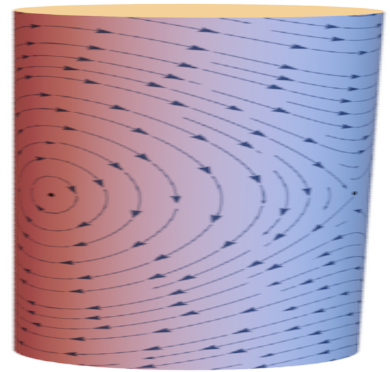
\includegraphics[width=.5\textwidth]{Pictures/pendulum_ham_PhaseSpace} 
		%https://mathematica.stackexchange.com/questions/64407/phase-portrait-on-a-cylinder
    \end{column}
    \begin{column}{.65\textwidth}	
		\begin{itemize}
			\item Interaction with the gravitational pull gives
				\vspace{-1em}			
				$$ H = \dfrac{p^2}{2 m \ell^2} + m	g \ell ( 1- \cos(\theta))$$
			\item 
				The corresponding Ham. v. f. results
				\vspace{-1em}				
				$$ X_H = - m g \ell \sin(\theta) \partial_p + \dfrac{p}{m \ell^2} \partial_\theta$$		
		\end{itemize}
  	\end{column}
	\end{columns}			
	\end{exblock}
	

\end{frame}
\note[itemize]{
	\item 	Recall: angular momentum $ p = m \ell \dot{\theta}$.
	\item Computing the flow of the Ham v.f. is where the analisys (exact solutions) or the numerics (approximate solutions) kicks in.
	\item why one should introduce all this machinery instead of going straight to the solution of the differential equations of motions?
		\begin{itemize}
			\item in quantization the global geometry of the system is more important then the local description of the classical motion
			\item efficient numerical schemes take in account the preservation of the symplectic form (do not solve the pde blindly but consider its geo-mech origin).
		\end{itemize}
}
%------------------------------------------------------------------------------------------------



\end{document}